\section{Shell Script - Syntax}

\begin{frame}[fragile]{Hello World}
\begin{multicols}{2}
\begin{itemize}
\item Open an editor and copy the following script:\\
\lstinputlisting[language=bash]{hello.sh}
\item Save it to a file (suppose it's \t{hello.sh}).
\newpage
\item Run it!
\begin{itemize}
\item First way: \t{bash hello.sh}
\item Second way: \t{chmod +x hello.sh} (remember to give it the execution permission)\\
\t{./hello.sh}
\item Result: 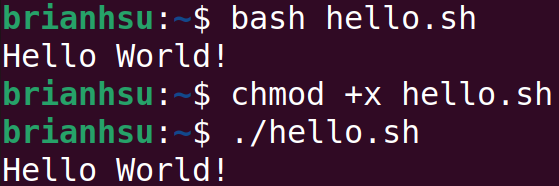
\includegraphics[width=5cm]{helloworld.png}
\end{itemize}
\end{itemize}
\end{multicols}
\end{frame}

\begin{frame}[fragile]{Shebang}
\begin{itemize}
\item Shebang (=Hashbang): sharp + bang
\item Specify the interpreter by adding shebang
\item \href{https://stackoverflow.com/questions/21612980/why-is-usr-bin-env-bash-superior-to-bin-bash}{\t{\#!/usr/bin/env bash} or \t{\#!/bin/bash}}
\item Python is also an interpreter: \t{\#!/usr/bin/env python}
\end{itemize}
\end{frame}

\begin{frame}[fragile]{Variables}
\begin{multicols}{2}
\begin{itemize}
\item Assign value (no spaces in the syntax): \t{var=value}\\
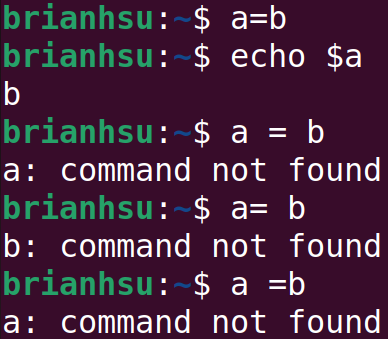
\includegraphics[width=3cm]{varassign.png}
\item Take value: \t{\$var}, \t{\$\{var\}}
\item echo with:
\begin{itemize}
\item Single quote: without replacement
\item Double quote: with replacement
\end{itemize}
\item \href{https://stackoverflow.com/questions/29378566/i-just-assigned-a-variable-but-echo-variable-shows-something-else}{I just assigned a variable, but \t{echo \$variable} shows something else}
\item Try this yourself:
\lstinputlisting[language=bash]{varex1.sh}
What is the output?
\end{itemize}
\end{multicols}
\end{frame}

\begin{frame}{Variables}
\begin{itemize}
\item Get the output of a command: \t{var=`cmd`}, \t{var=\$(cmd)}
\item Get the exit code of the last command: \t{var=\$?}
\item Exit with a specific exit code: \t{exit code}
\item Calculation
\begin{itemize}
\item String concatenation: \t{\$a\$b}
\item Integer Arithmetic: \t{\$((a+b))}, \t{((a*=b))}, \t{((++a))}, \t{((a-=1))}
\item String length: \t{\$\{\#a\}}
\end{itemize}
\end{itemize}
\end{frame}

\begin{frame}[fragile]{Variables - Array}
\begin{multicols}{2}
\begin{itemize}
\item Declare an array (IFS-sep): \t{arr=("a" "b")}, \t{files=(`ls`)}
\item Append to an array: \t{arr+=("c")}
\item Assign: \t{arr[i]=value}
\item Get the values of an array:
\begin{itemize}
\item All items in \t{arr}: \t{\$\{arr[@]\}}
\item The size of \t{arr}: \t{\$\{\#arr[@]\}}
\item The value of \t{arr[i]}: \t{\$\{arr[i]\}}
\end{itemize}
\item Get the values of the arguments (can be seen as an array):
\begin{itemize}
\item The argument of a script: \t{\$1}, \t{\$2}, \dots
\item All arguments of a script: \t{\$@}
\item The number of arguments: \t{\$\#}
\end{itemize}
\item IFS (Internal Field Separator) (like \t{.split()} in python): \t{IFS=\$' \symbol{92}t\symbol{92}n'} by default
\end{itemize}
\end{multicols}
\end{frame}

\begin{frame}[fragile]{Variables - Array}
\begin{itemize}
\item Try the following code in a directory with more than 2 files.
\lstinputlisting[language=bash]{array.sh}
Save it to \t{script.sh} and run \t{./script.sh 12 34}.
\end{itemize}
\end{frame}

\begin{frame}{Variables - Dictionary}
\begin{itemize}
\item Declare with attributes: \t{declare [attribute-option] var=value}
\item Delete a variable: \t{unset var}
\item Declare a dictionary: \t{declare -A dict}, \t{dict=([abc]=def [123]='456')}
\item Assign: \t{dict[key]=value}
\item Get the values of an dictionary:
\begin{itemize}
\item All items in \t{dict}: \t{\$\{dict[@]\}}
\item The size of \t{dict}: \t{\$\{\#dict[@]\}}
\item The value of \t{dict[key]}: \t{\$\{dict[key]\}}
\end{itemize}
\item \href{https://www.howtogeek.com/730243/what-are-bash-dictionaries-on-linux-and-how-do-you-use-them/}{What Are Bash Dictionaries on Linux, and How Do You Use Them?}
\end{itemize}
\end{frame}

\begin{frame}[fragile]{Redirection}
\begin{multicols}{2}
\begin{itemize}
\item Input into a variable: \t{read var}
\item Redirection:
\begin{itemize}
\item \t{<}: redirect STDIN to file
\item \t{>}: redirect STDOUT to file (cover)
\item \t{>>}: redirect STDOUT to file (append)
\item \t{2>}: redirect STDERR to file
\item \t{\&>}: redirect STDOUT and STDERR to file
\item \t{>\&}: redirect a stream to another
\end{itemize}
\newpage
\item What is the output and the content of each file after running the following code?
\lstinputlisting[language=bash]{redirect.sh}
\end{itemize}
\end{multicols}
\end{frame}

\begin{frame}[fragile]{Redirection}
\begin{itemize}
\item \t{cmd1 | cmd2}: pass the STDOUT of \t{cmd1} to the STDIN of \t{cmd2}\\
The following do almost the same thing:
\begin{itemize}
\item \t{cat messy.txt | sort | uniq > clean.txt}
\item \t{cat messy.txt > tmp1; sort < tmp1 > tmp2}\\
\t{uniq < tmp2 > clean.txt; rm tmp1 tmp2}
\end{itemize}
\item \t{cmd1; cmd2; ...}: use \t{;} to split the commands in a single line
\item \t{cmd <<< str}: here-string, like redirecting STDIN to \t{str}
\item \t{cmd \&}: run \t{cmd} in background
\end{itemize}
\end{frame}
